% !TEX root = ../algo-summary.tex
\section{Greedy Algorithms}\label{sec:greedy_algorithms}

\subsection{Interval Scheduling}
Given \(n\) jobs, we want to schedule a maximum number of non-overlapping jobs, i.e.
\begin{itemize}
  \item Job \(j\) starts at \(s_j\) and finishes at \(f_j\)
  \item Two jobs are \hl[2]{compatible} if they don't overlap
  \item Goal: find a \emph{maximum cardinality} subset of mutually compatible jobs
\end{itemize}


greedy template:
Consider jobs in some order.
Take a job if it is compatible with all previously selected jobs.

What order?
\begin{itemize}
\item (Earliest start time) ascending order of start time ${s}_{{j}}$.
\item (Shortest interval) ascending order of interval length $f_j-s_j$.
\item (Fewest conflicts) 
for each job, count the number of conflicting jobs ${c}_{{j}}$. 
ascending order of conflicts ${c}_{{j}}$.
\item (Earliest finish time) ascending order of finish time $f_j$.
\end{itemize}
all of the above are valid thoughts, but can easily find counterexample for the first three of them:
\[
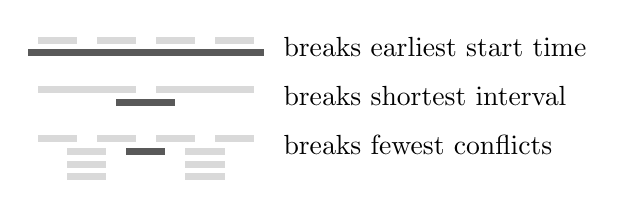
\begin{tikzpicture}[scale=0.25]
\definecolor{L}{gray}{0.85}
\definecolor{D}{gray}{0.35}
\def\h{0.35}

% ------------------ breaks earliest start time ------------------
\begin{scope}[shift={(0,5)}]
  \fill[L] (0,0.15) rectangle ++(2,\h);
  \fill[L] (3,0.15) rectangle ++(2,\h);
  \fill[L] (6,0.15) rectangle ++(2,\h);
  \fill[L] (9,0.15) rectangle ++(2,\h);
  \fill[D] (-0.5,-0.15) rectangle ++(12,-\h);
  \node[anchor=west] at (12,0) {breaks earliest start time \textcolor{red}{\Lightning}};
\end{scope}

% ------------------ breaks shortest interval ------------------
\begin{scope}[shift={(0,2.5)}]
  \fill[L] (0,0.15) rectangle ++(5,\h);
  \fill[L] (6,0.15) rectangle ++(5,\h);
  \fill[D] (4,-0.15) rectangle ++(3,-\h);
  \node[anchor=west] at (12,0) {breaks shortest interval \textcolor{red}{\Lightning}};
\end{scope}

% ------------------ breaks fewest conflicts ------------------
\begin{scope}[shift={(0,0)}]
  % top row
  \fill[L] (0,0.15) rectangle ++(2,\h);
  \fill[L] (3,0.15) rectangle ++(2,\h);
  \fill[L] (6,0.15) rectangle ++(2,\h);
  \fill[L] (9,0.15) rectangle ++(2,\h);
  % second row
  \fill[L] (1.5,-0.15) rectangle ++(2,-\h);
  \fill[D] (4.5,-0.15) rectangle ++(2,-\h);
  \fill[L] (7.5,-0.15) rectangle ++(2,-\h);
  % third row
  \fill[L] (1.5,-0.8) rectangle ++(2,-\h);
  \fill[L] (7.5,-0.8) rectangle ++(2,-\h);
  % fourth row
  \fill[L] (1.5,-1.45) rectangle ++(2,-\h);
  \fill[L] (7.5,-1.45) rectangle ++(2,-\h);
  \node[anchor=west] at (12,0) {breaks fewest conflicts \textcolor{red}{\Lightning}};
\end{scope}

\end{tikzpicture}
\]


(a correct) greedy strategy: 
increasing order of finish time \textcolor{Green}{\ding{52}}
% Take a job if it is compatible with all previously selected jobs.

or symmetrically:
decreasing order of start time \textcolor{Green}{\ding{52}}

\begin{algorithm}[h]
\caption{Greedy Interval Scheduling}\label{alg:greedy_interval_scheduling}
\begin{algorithmic}[1]
\State sort jobs by finish time: \(f_1 \le f_2 \le \ldots \le f_n\)
\State $A\gets\emptyset$ \Comment{selected jobs}
\For{$j=1 \TO n$}
  \If{job \(j\) is compatible with (last) job in \(A\)}
    \State $A\gets A\cup\{j\}$
  \EndIf
\EndFor
\State \Return $A$
\end{algorithmic}
\end{algorithm}


Implementation. \(O(n\log n)\) for sorting
\begin{itemize}
\item remember job \(j^*\) that was added last to \(A\)
\item job \(j\) is compatible with \(A\) if \(s_j \geq f_{j^*}\)
\end{itemize}


\begin{theorem}[Optimality]\label{thm:greedy_interval_scheduling_optimality}
\autoref{alg:greedy_interval_scheduling} is optimal.
\end{theorem}
\begin{proof}
Consider an optimal schedule \(O\), and let \(G\) be the greedy schedule.
Let \(O = [x_1, x_2, \ldots, x_k]\) the activities of \(O\) listed in increasing order of finish time,
and let \(G = [g_1, g_2, \ldots, g_{k'}]\) be the corresponding greedy schedule.
If \(G = O\), we are done.
Otherwise, let \(j\) be the first index where \(x_j \neq g_j\), i.e.
\[
\begin{aligned}
O &= [x_1, x_2, \ldots, x_{j-1}, {x_j}, x_{j+1}, \ldots, x_k] \\
G &= [x_1, x_2, \ldots, x_{j-1}, {g_j}, g_{j+1}, \ldots, g_{k'}]
\end{aligned}
\]
where \(g_j \neq x_j\).
Note that \(k \geq j\) since otherwise \(G\) would have more activities than \(O\), contradictory.
\autoref{alg:greedy_interval_scheduling} selects the the activity with the earliest finish time that does not conflicct with any earlier activity.
Thus, we know that \(g_j\) does not conflict with any earlier activity, and it finishes no later than \(x_j\) finishes:
\[
\begin{tikzpicture}[>=Stealth, scale=0.5, font=\footnotesize]
  \tikzset{
    box/.style={draw, minimum width=0.9cm, minimum height=0.28cm,
                inner sep=0pt, align=center, anchor=west},
    gbox/.style={box, fill=gray!30},
    boxsmall/.style={draw, minimum width=0.6cm, minimum height=0.28cm,
                     inner sep=0pt, align=center, anchor=west},
    gboxsmall/.style={boxsmall, fill=gray!30}
  }

  % left-edge x positions of columns
  \def\xA{1.0}
  \def\xB{3.0}
  \def\xC{5.35}
  \def\xD{6.2}
  \def\xE{8.2}
  \def\xF{10.2}
  \def\xG{12.2}
  \def\xH{14.45}

  % y-positions for the rows
  \def\yO{0.0}
  \def\yG{-0.8}
  \def\yLine{-1.4}
  \def\yOp{-2.0}

  % Row labels
  \node at (0,\yO) {$O:$};
  \node at (0,\yG) {$G:$};
  \node at (0,\yOp) {$O':$};

  % --- Row O ---------------------------------------------------------------
  \node[box] at (\xA,\yO) {$x_1$};
  \node[box] at (\xB,\yO) {$x_2$};
  \node      at (\xC+0.2,\yO) {$\cdots$};
  \node[box] at (\xD,\yO) {$x_{j-1}$};
  \node[box] at (\xE,\yO) {$x_j$};
  \node[box] at (\xF,\yO) {$x_{j+1}$};
  \node[box] at (\xG,\yO) {$x_{j+2}$};
  \node      at (\xH,\yO) {$\cdots$};

  % --- Row G ---------------------------------------------------------------
  \node[box]       at (\xA,\yG) {$x_1$};
  \node[box]       at (\xB,\yG) {$x_2$};
  \node            at (\xC+0.2,\yG) {$\cdots$};
  \node[box]       at (\xD,\yG) {$x_{j-1}$};
  \node[gboxsmall] at (\xE,\yG) {$g_j$};      % left edges aligned with x_j column
  \node[gbox]      at (\xF-0.6,\yG) {$g_{j+1}$};
  \node[gbox]      at (\xG-0.6,\yG) {$g_{j+2}$};
  \node            at (\xH-0.6,\yG) {$\cdots$};

  % Divider
  \draw (0.0,\yLine) -- (\xH+0.6,\yLine);

  % --- Row O' --------------------------------------------------------------
  \node[box]  at (\xA,\yOp) {$x_1$};
  \node[box]  at (\xB,\yOp) {$x_2$};
  \node       at (\xC+0.2,\yOp) {$\cdots$};
  \node[box]  at (\xD,\yOp) {$x_{j-1}$};
  \node[gboxsmall] at (\xE,\yOp) {$g_j$};          % same left edge as above
  \node[box]  at (\xF,\yOp) {$x_{j+1}$};
  \node[box]  at (\xG,\yOp) {$x_{j+2}$};
  \node       at (\xH,\yOp) {$\cdots$};

  % Curved arrow on the left
  \draw[->, line cap=round] (-0.6,\yO) .. controls ($(-1,-0.5)$) and ($(-1,-1.5)$) .. (-0.6,\yOp);
\end{tikzpicture}
\]

Consider the the modified `greedier' schedule \(O'\) obtained by replacing \(x_j\) with \(g_j\) in \(O\).
That is, 
\[
O' = [x_1, x_2, \ldots, x_{j-1}, {g_j}, x_{j+1}, \ldots, x_k]
\]
it is a valid schedule, because \(g_j\) finishes no later than \(x_j\) and therefore cannot create any new conflicts.
It has the same \(\numof\)activities as \(O\), so it is at least as good.
By repeating this process, we will eventually convert \(O\) into \(G\) without ever decreasing the number of activities.
Thus, \(G\) is optimal.
\end{proof}






\subsection{Interval Partitioning}
Given \(n\) jobs, we want to schedule them all using a minimum number of resources (e.g., classrooms), i.e.
\begin{itemize}
  \item Job \(j\) starts at \(s_j\) and finishes at \(f_j\)
  \item Goal: find a \emph{minimum number} of resources (e.g., classrooms) to schedule all jobs
\end{itemize}

\begin{definition}[depth]\label{def:depth}
The \emph{depth} of a set of open intervals is the maximum number that contain any given time (vertical line), i.e.
\[
\text{depth} = \max_{t} A(t)
\]
where \(A(t)\) is the number of intervals that contain (i.e. that are \emph{active} at time \(t\)).
\end{definition}
Key observation: \(d\) \(=\) \(\numof\)resources \(\geq\) depth

Greedy strategy: 
Consider jobs in increasing order of start time.
Assign job to any compatible resource, or open a new resource.


\begin{algorithm}[h]
\caption{Greedy Interval Partitioning}\label{alg:greedy_interval_partitioning}
\begin{algorithmic}[1]
\State sort jobs by starting time: \(s_1 \le s_2 \le \ldots \le s_n\)
\State \(d \gets 0\) \Comment{number of allocated resources}
\For{$j=1 \TO n$}
  \If{job \(j\) is compatible some available resource \(k\)}
    \State schedule job \(j\) on resource \(k\)
  \Else
    \State allocate a new resource \(d + 1\)
    \State schedule job \(j\) on resource \(d + 1\)
    \State \(d \gets d + 1\)
  \EndIf
\EndFor
\end{algorithmic}
\end{algorithm}


Implementation. \(O(n\log n)\) 
\begin{itemize}
\item sort takes \(O(n\log n)\) 
\item for each ressource \(k\), maintain the finish time of the last job added 
\item avoid quadratic algorithm (scanning all allocated \(d\) resources every single time) 
\item first idea: priority queue (min-heap) of ressources, keyed by time they become free
\item interact with the heap in \(O(\log d)\) time per job: get-min, del-min, insert
\end{itemize}

But actually, we can do better (for the part after sorting): 
\begin{itemize}
\item maintain a stack/queue \(Q\) of available resources 
\item initially \(Q\) is empty 
\item create a sorted list of \(2n\) \hl{job events}: 
turn every interval \([s_i, f_i)\) into two events  
\((s_i, \texttt{start})\) and \((f_i, \texttt{finish})\). 
finish events come before start events at the same time 
(lets a job ending at time \(t\) free a room that a job starting at time \(t\) can immediately reuse).  
\item at a start event a ressource is allocated from \(Q\) (or a new one (\(+\!+\!d\)) is created if \(Q\) is empty) 
\item at a finish event, a ressource is freed and put back onto \(Q\) 
\item \textcolor[HTML]{013399}{principle of 1D plane sweep by vertical line from left to right}
\end{itemize}

\begin{theorem}[Optimality]\label{thm:greedy_interval_partitioning_optimality}
\autoref{alg:greedy_interval_partitioning} is optimal.
\end{theorem}
\begin{proof}
We can show that ${d} \leq \text{depth}$ (enough to prove optimality):
\begin{itemize}
\item Ressource $d$ is allocated because we needed to schedule a job $j$ that is incompatible with all the current ${d}-1$ ressources, which hold jobs that started before ${s}_{j}$ (no later than ${s}_{j}$) and none has finished yet.
\item Consider time ${s}_{j}+\varepsilon$. At that time $({d}-1)+1={d}$ intervals are overlapping and since since depth is the maximum number of overlapping intervals at any time, we have ${d} \leq \text{depth}$.
\qedhere
\end{itemize}
\end{proof}



\subsection{Minimizing Lateness}\label{sec:minimizing_lateness}
Given \(n\) jobs, where
\begin{itemize}
  \item job \(j\) requires \(t_j\) units processing time and is due at \(d_j\) (deadline)
  \item if job \(j\) starts at time \(s_j\), it finishes at \(f_j = s_j + t_j\)
  \item lateness: \(\ell_j = \max(0, f_j - d_j)\) \hspace{1em} \textcolor{green}{finish time - deadline}
  \item goal: schedule all jobs to \emph{minimize} \hl[2]{maximum lateness} \(L = \max_j \ell_j\)
\end{itemize}

greedy template:
Consider jobs in some order.
\begin{itemize}
\item (Shortest processing time) ascending order of processing time ${t}_{j}$.
\item (Earliest deadline) ascending order of deadlines ${d}_{j}$.
\item (Smallest slack) ascending order of slack time $s_j = d_j - t_j$
\end{itemize}

but there are problems for first and last:
\begin{itemize}
\item short job may have a long deadline, e.g. \([(t_1,d_1)=(1,100),(t_2,d_2)=(10,10)]\) \textcolor{red}{\Lightning}
\item long job may have \(0\) slack, e.g. \([(t_1,d_1)=(1, 2),(t_2,d_2)=(10,10)]\) \textcolor{red}{\Lightning}
\end{itemize}

the correct greedy strategy is: earliest deadline first \textcolor{Green}{\ding{52}}
\begin{algorithm}[h]
% \begin{aligned}
% &\text { Sort } \mathrm{n} \text { jobs by deadline so that } \mathrm{d}_1 \leq \mathrm{d}_2 \leq \ldots \leq \mathrm{d}_{\mathrm{n}}\\
% &\mathrm{t} \leftarrow 0\\
% &\text { for j = } 1 \text { to n }\\
% &\text { Assign job j to interval [ } t, t+t_j \text { ] }\\
% &\mathbf{s}_{\mathbf{j}} \leftarrow \mathbf{t}, \mathbf{f}_{\mathbf{j}} \leftarrow \mathbf{t}+\mathbf{t}_{\mathbf{j}}\\
% &\mathrm{t} \leftarrow \mathrm{t}+\mathrm{t}_{\mathrm{j}}\\
% &\text { output intervals }\left[\mathrm{s}_{\mathrm{j}}, \mathrm{f}_{\mathrm{j}}\right]
% \end{aligned}
\caption{Greedy Minimizing Lateness}\label{alg:greedy_minimizing_lateness}
\begin{algorithmic}[1]
\State sort jobs by deadline: \(d_1 \le d_2 \le \ldots \le d_n\)
\State $t \gets 0$ \Comment{current time}
\For{$j=1 \TO n$}
  \State assign job \(j\) to interval \([t, t+t_j]\)
  \State $s_j \gets t$
  \State $f_j \gets t+t_j$
  \State $t \gets t+t_j$
\EndFor
\Return intervals \([s_j, f_j]\)
\end{algorithmic}
\end{algorithm}



\begin{observation}\label{obs:exists_optimal_no_idle}
There exists an optimal schedule with no \textcolor[HTML]{CC0100}{idle time} (idle time gives no benefit).
\end{observation}

\begin{observation}\label{obs:greedy_no_idle}
The \hyperref[alg:greedy_minimizing_lateness]{greedy schedule} has no idle time (by construction).
\end{observation}

\begin{definition}[inversion]\label{def:inversion}
An inversion in schedule \(S\) is a pair of jobs \(i,j\) such that \(d_i < d_j\) but \(j\) is scheduled before \(i\).
\end{definition}

\begin{observation}\label{obs:greedy_no_inversion}
The \hyperref[alg:greedy_minimizing_lateness]{greedy schedule} has no inversions (by construction - ascending order of deadlines).
\end{observation}

\begin{observation}\label{obs:inversion_implies_consecutive_iversion}
If a schedule (with no idle time) has an inversion, there is an inversion with two inverted jobs scheduled consecutively.
\end{observation}

\begin{claim}
\label{claim:swap_does_not_increase_lateness}
Swapping two adjacent inverted jobs reduces number of inversions by \(1\) and does not increase the max lateness \(\ell_{\max} := \max \{\ell_1, \ldots, \ell_n\}\).
\end{claim}

\begin{proof}
Let \(\ell\) be the lateness before the swap and let \(\ell'\) be it after the swap.
\begin{itemize}
  \item \(\ell_k' = \ell_k\) for all \(k \neq i,j\) (no change)
  \item \(\ell_i' \leq \ell_i\) because \(i\) finishes earlier after the swap
  \item if job \(j\) was late before the swap: 
  \[
  \begin{aligned}
    \ell_j' &= f_j' - d_j &&\text{(definition)} \\
            &= f_i - d_j &&\text{(\(j\) now finishes when \(i\) used to finish)} \\
            &\leq f_i - d_i &&\text{(since \(d_i < d_j\))} \\
            &= \ell_i &&\text{(definition)}
  \end{aligned}
  \]
  \end{itemize}
\[
\begin{tikzpicture}[scale=0.5,
  >={Latex[length=1mm, width=1mm]},
  lab/.style={font=\footnotesize, text height=1ex, text depth=0pt, baseline}
]

\def\labelpos{0.9}
\def\dipos{1}
\def\djpos{2}
\def\sjpos{3.5}
\def\mpos{5}
\def\fipos{7}

\def\blockh{0.7}     % block height


\node[lab, anchor=east] at (\labelpos,\blockh/2) {before swap:};

% jobs
\node at (\sjpos-0.5,\blockh/2) {$\cdots$};
\draw[draw=black, fill=gray!35] (\sjpos,0) rectangle (\mpos,\blockh);
\node[lab] at ({(\sjpos+\mpos)/2},\blockh/2) {$j$};
\draw[draw=black, fill=gray!35] (\mpos,0) rectangle (\fipos,\blockh);
\node[lab] at ({(\mpos+\fipos)/2},\blockh/2) {$i$};
\node at (\fipos+0.5,\blockh/2) {$\cdots$};
\draw[<->] (\sjpos,\blockh+0.2) -- (\mpos,\blockh+0.2) node[midway,above,lab] {$t_j$};
\draw[<->] (\mpos,\blockh+0.2) -- (\fipos,\blockh+0.2) node[midway,above,lab] {$t_i$};

% deadlines (d_i < d_j)
\draw[densely dotted] (\dipos,-2) -- (\dipos,1);
\draw[] (\dipos,1) -- (\dipos,1.2) node[lab, above] {$d_i$};
\draw[densely dotted] (\djpos,-1.2) -- (\djpos,1);
\draw[] (\djpos,1) -- (\djpos,1.2) node[lab, above] {$d_j$};

% finish times
\draw[densely dotted] (\mpos,-1.2) -- (\mpos,0);
\draw[densely dotted] (\fipos,-2) -- (\fipos,0);

% lateness
\draw[<->] (\djpos,-1) -- (\mpos,-1) node[lab, midway, above] {$\ell_j$};
\draw[<->] (\dipos,-1.8) -- (\fipos,-1.8) node[lab, midway, above] {$\ell_i$};


\begin{scope}[shift={(12,0)}]
\def\labelpos{0.9}
\def\dipos{1}
\def\djpos{2}
\def\sipos{3.5}
\def\mpos{5.5}
\def\fjpos{7}

\def\blockh{0.7}     % block height

\node[lab, anchor=east] at (\labelpos,\blockh/2) {after swap:};

% jobs
\node at (\sipos-0.5,\blockh/2) {$\cdots$};
\draw[draw=black, fill=gray!35] (\sipos,0) rectangle (\mpos,\blockh);
\node[lab] at ({(\sipos+\mpos)/2},\blockh/2) {$i$};
\draw[draw=black, fill=gray!35] (\mpos,0) rectangle (\fjpos,\blockh);
\node[lab] at ({(\mpos+\fjpos)/2},\blockh/2) {$j$};
\node at (\fjpos+0.5,\blockh/2) {$\cdots$};
\draw[<->] (\sipos,\blockh+0.2) -- (\mpos,\blockh+0.2) node[midway,above,lab] {$t_i$};
\draw[<->] (\mpos,\blockh+0.2) -- (\fjpos,\blockh+0.2) node[midway,above,lab] {$t_j$};

% deadlines (d_i < d_j)
\draw[densely dotted] (\dipos,-2) -- (\dipos,1);
\draw[] (\dipos,1) -- (\dipos,1.2) node[lab, above] {$d_i$};
\draw[densely dotted] (\djpos,-1.2) -- (\djpos,1);
\draw[] (\djpos,1) -- (\djpos,1.2) node[lab, above] {$d_j$};

% finish times
\draw[densely dotted] (\fjpos,-1.2) -- (\fjpos,0);
\draw[densely dotted] (\mpos,-2) -- (\mpos,0);

% lateness
\draw[<->] (\djpos,-1) -- (\fjpos,-1) node[lab, midway, above] {$\ell_j'$};
\draw[<->] (\dipos,-1.8) -- (\mpos,-1.8) node[lab, midway, above] {$\ell_i'$};
\end{scope}

\end{tikzpicture}
\]

Thus we have \(
 \ell_{\max}' = \max{\{\ell_i', \ell_j', \text{others}\}} \leq \max{\{\ell_i, \text{others}\}} = \ell_{\max}
\).
\end{proof}

\begin{theorem}[Optimality]\label{thm:greedy_minimizing_lateness_optimality}
\autoref{alg:greedy_minimizing_lateness} is optimal.
\end{theorem}
\begin{proof}
Let \(G\) be the greedy schedule produced by \autoref{alg:greedy_minimizing_lateness}.
Let \(O\) be an optimal schedule with the fewest number of inversions.
We can assume \(O\) has no idle time.
If \(O\) has no inversions, then \(O = G\).
Otherwise, let \(i,j\) be two adjacent inverted jobs in \(O\).
By \autoref{claim:swap_does_not_increase_lateness}, swapping \(i\) and \(j\) does not increase the maximum lateness and strictly decreases the number of inversions.
This contradicts the definition of \(O\). \textcolor{red}{\Lightning}
\end{proof}

Alternatively, we can prove \autoref{thm:greedy_minimizing_lateness_optimality} using an exchange argument:
We can take \(O\) and transform into \(G\) by removing inversions 1 by 1 with no change in max lateness.


\subsection{Analysis Strategies and Approximation}

\subsubsection{Correctness Proofs}
\textcolor[HTML]{013399}{Greedy algorithm stays ahead}.
Show that after each step of the greedy algorithm, its solution is at least as good as any other algorithm's.

\textcolor[HTML]{013399}{Exchange argument}.
Gradually transform any solution to the one found by the greedy algorithm without hurting its quality.

\textcolor[HTML]{013399}{Structural}.
Discover a simple "structural" bound asserting that every possible solution must have a certain value. 
Then show that your algorithm always achieves this bound.

\textcolor[HTML]{013399}{Counterexample}.
To show that a greedy algorithms does \emph{not} work, all we need is a small counterexample.


\subsubsection{Greedy Approximation for NP-Hard Problems}

The greedy approach is not very powerful as an algorithm design technique.
\begin{itemize}
  \item One of most common applications of greedy algorithms is to produce approximation solutions to NP-hard problems.
  \item NP-hard optimization problems are challenging computational problems with no known exact solution of worst-case polynomial-time running time.
  \item Given an NP-hard problem, there are no ideal solutions. Compromise between optimality or running time.
  \item Instances of such problems where simple greedy algorithms produce solutions that are not far from optimal. E.g., clustering and Facility Location.
\end{itemize}


\subsection{Shortest Paths}\label{sec:shortest_paths}

\textcolor[HTML]{013399}{Shortest path network}.
\begin{itemize}
  \item directed of undirected graph \(G=(V,E)\)
  \item source \(s\), destination/target \(t\)
  \item length/weight function \(w:E\to\R\) (assigns cost/length to each edge)
\end{itemize}

\textcolor[HTML]{013399}{Shortest path problem}: find shortest (directed) path from \(s\) to \(t\).






\subsubsection*{\nameref{alg:dijkstra}'s algorithm}
%  is a greedy, label-setting method for nonnegative edge weights.  
% At each step it finalizes the closest unreached vertex and relaxes its outgoing edges, yielding a time complexity of \(O(( n+m)\log  n)\) with a binary-heap implementation.

\begin{itemize}
  \item assume \hypertarget{non_negative_assumption}{\(w(e) \geq 0\)} for all edges \(e\) (non-negative weights)
  \item maintain a set of \textcolor[HTML]{CC0100}{explored nodes \(S\)} for which we have determined the the \hl{shortest path distance \(\attribnormal{u}{\delta}\)} from \(s\) to \(u\)
  \item initialize \(S = \{s\}\) and \(\attribnormal{s}{\delta} = 0\)
  \item repeatedly choose unexplored node \(v\) which minimizes 
  \begin{equation}\label{eq:dijkstra_ds}
  d_S(v) := \min_{e=(u,v), u\in S} \left(\attrib{u}{\delta} + w(e)\right)
  \end{equation}
  where \(d_S(v)\) is the shortest path to some \(u\) in explored part \(S\), followed by a single edge \((u,v)\), i.e.
  it is the shortest path from \(s\) to \(v\) using only vertices in \(S\).
  Add \(v\) to \(S\) and set \(\attrib{v}{\delta} = d_S(v)\).
\end{itemize}

two sets of vertices: \(S\) (explored nodes) and \(V\setminus S\) (unexplored)
\begin{itemize}
  \item \(V \setminus S\) organized in a priority queue \(Q\) (heap of min \(d\) value)
  \item vertices in \(Q\) have weight \(d_S(v)\): length of shortest path to \(v\) using only vertices in \(S\)
  \item vertices in \(S\) have weight \(\attrib{u}{\delta}\): length of shortest \(s\)-\(u\) path
  \item every time a vertex \(u\) gets explored (joins \(S\)), we \hl[2]{``relax'' all incident edges \((u,v)\)}:
        for all vertices \(v\) adjacent to \(u\):
        update \(d_S(v)\) to \(\min(d_S(v), \attrib{u}{\delta} + w(u,v))\)
  \item next node to explore = node with minimum \(d_S(v)\) 
\end{itemize}

\textcolor[HTML]{013399}{Efficient implementation}.
Maintain a priority queue of unexplored nodes, prioritized by \(d_S(v)\).


\begin{table}[ht]
  \centering
  \renewcommand{\arraystretch}{1.1}
  \begin{tabular}{
    p{0.18\textwidth}  % a bit wider first column
    |  
    >{\centering\arraybackslash}p{0.12\textwidth}
    >{\centering\arraybackslash}p{0.14\textwidth}
    >{\centering\arraybackslash}p{0.14\textwidth}
    >{\centering\arraybackslash}p{0.14\textwidth}
    >{\centering\arraybackslash}p{0.14\textwidth}
  }
    \toprule
    {PQ Operation} & {Dijkstra} & {Array} & {Binary heap} & {d-way Heap} & {Fib heap}$^{\hyperlink{table_footnote}{\dagger}}$ \\
    \midrule
    Insert     & $n$ & $n$ & $\log n$ & $d \log_{d} n$ & $1$ \\
    ExtractMin & $n$ & $n$ & $\log n$ & $d \log_{d} n$ & $\log n$ \\
    ChangeKey  & $m$ & $1$ & $\log n$ & $\log_{d} n$ & $1$ \\
    IsEmpty    & $n$ & $1$ & $1$ & $1$ & $1$ \\
    \midrule
    \textbf{Total} &  & $n^{2}$ & $m \log n$ & $m \log_{m/n} n$ & $m + n \log n$ \\
    \bottomrule
  \end{tabular}
  \vspace{0.5em}
  {\footnotesize \hypertarget{table_footnote}{$^{\dagger}$ Individual operations are amortized bounds.}}
\end{table}


\begin{algorithm}[h]
\caption{Dijkstra}\label{alg:dijkstra}
\begin{algorithmic}[1]
\Function{Dijkstra}{$G, w:E\to\R_{\textcolor{red}{\ge 0}}, s$} 
  \ForAll{$v\in V$} \Comment{initialization}
    \State $\attrib{v}{\delta}\gets\infty$ \Comment{best known cost from \(s\) to \(v\)}
    \State $\attrib{v}{color} \gets \text{undiscovered}$
    \State $\attrib{v}{\pi}\gets\nil$ \Comment{node preceding \(v\) on the least-cost path from \(s\)}
  \EndFor
  \State $\attrib{s}{\delta}\gets 0$ \Comment{\(s\) is the source}
  \State $Q \gets $ priority queue of all nodes \(u \in V\) sorted by \(\attrib{u}{\delta}\)
  \While{$Q \neq \emptyset$} \Comment{until all vertices are processed}
    \State extract \(u\) with minimal \(\attrib{u}{\delta}\) from \(Q\) \label{line:dijkstra_extract_min}
    \ForAll{$v\in\Gamma(u)$}
      \If{$\attrib{u}{\delta} + w(u,v) < \attrib{v}{\delta}$} \Comment{relax edge \((u,v)\), i.e. update \hyperref[eq:dijkstra_ds]{\(d_S(v)\)}}
        \State $\attrib{v}{\delta} \gets \attrib{u}{\delta} + w(u,v)$
        \State decrease key of \(v\) in \(Q\) to \(\attrib{v}{\delta}\)
        \State $\attrib{v}{\pi} \gets u$
      \EndIf
    \EndFor
    \State $\attrib{u}{color} \gets \text{finished}$
  \EndWhile
  \LComment{the \(\attribute{\pi}\) pointers define an `inverted' shortest path tree}
\EndFunction
\end{algorithmic}
\end{algorithm}



\textcolor[HTML]{013399}{Time analysis (using a binary heap)}.
\begin{itemize}
  \item extract a vertex \(u\) from priority queue \(Q\): \(O(\log n)\)
  \item for each incidnt edge \((u,v)\), relax it in \(O(1)\) and spend \(O(\log n)\) if we decrease the key of \(v\) in \(Q\) 
\end{itemize}
Thus, time to process vertex \(u\) is \(O(\log n + \deg(u) \log n)\) and total time is
\[
\begin{aligned}
T(n, m) &= \sum_{u \in V} (\log n + \deg(u) \log n) \\
&= \log n \sum_{u \in V} (1 + \deg(u)) \\
&= (\log n) (n + 2m) \\
&= O((n + m) \log n)
\end{aligned}
\]


\begin{observation}\label{obs:attribute_d}
For all \(u \in V \setminus S\) we have
\[
\attrib{u}{\delta} = d_S(u)
\]
i.e. the key in the PQ is exactly \(d_S(u)\).
\end{observation}

\begin{caution}
We use the same variable/attribute \(\attrib{u}{\delta}\) to store both \(d_S(u)\) for the \(u \in V \setminus S\) and `later' \(\delta(s, u)\) for the \(u \in S\).

Only once a vertex \(u\) is extracted from the queue \(Q\) in Line \ref{line:dijkstra_extract_min} (which means it is added to \(S\)), we are guaranteed that \(\attrib{u}{\delta} = \delta(s, u)\).
\end{caution}

\begin{theorem}\label{thm:dijkstra_correctness}
For all \(u \in S\) we have
\[
\attrib{u}{\delta} = \delta(s, u)
\]
i.e. it is the length of the shortest \(s\)-\(u\) path.
\end{theorem}

\begin{proof}[Induction on \(|S|\)]\label{proof:dijkstra_correctness}
\leavevmode
\begin{enumerate}[partopsep=0em, label=(\roman*)]
\item Base case:
\(|S|=1\) is trivial: \(\attrib{u}{\delta} = \attrib{s}{\delta} = 0\) \textcolor{Green}{\ding{52}}
\item Induction hypothesis:
Assume true for \(|S| = k \geq 1\). 
\label{proof:dijkstra_correctness:induction_hypothesis}
\item Induction step:
Prove true for \(|S| = k+1\).

Let \(v\) be the \((k+1)^{\text{th}}\) node added to \(S\), and let \((u,v)\) be the chosen edge, and therefore \(\attrib{v}{\delta} = \attrib{u}{\delta} + w(u,v)\).
% We need to show that in that case \(\attrib{v}{\delta} = \delta(s,v)\).

Consider any \(s\)-\(v\) path \(P\):
  \[
\begin{tikzpicture}[>=Stealth, scale=0.4, font=\footnotesize]
\useasboundingbox (-3,-2.5) rectangle (5,2.5);
% background blob
\fill[black!20] plot[smooth cycle,tension=0.7] coordinates {(-3.4,1.5) (-2.0,2.3) (-0.4,2.0) (1.6,2.2) (3.6,1.6) (4.5,0.7) (5.1,-0.2) (4.6,-1.3) (3.2,-2.1) (1.3,-2.3) (-0.6,-2.0) (-2.2,-1.7) (-3.2,-0.8)};
\node at (-2.75,1.5) {\(S\)};
% nodes
\tikzset{state/.style={circle,draw,fill=white,minimum size=9pt,inner sep=0pt}}
\node[state] (s) at (-1.5,0.0) {\(s\)};
\node[state] (x) at (3.3,0.5)  {\(x\)};
\node[state] (y) at (5.5,1.5)  {\(y\)};
\node[state] (u) at (2.4,-1.5) {\(u\)};
\node[state] (v) at (5.2,-2) {\(v\)};
% paths
\draw[-, rounded corners=3pt, blue] (s) -- (-0.2, 1.2) -- (0.9, 0.4) node[midway, right, yshift=0.08cm] {$P'$} -- (2.0, 1.2) -- (x) ; % s -> x (P')
\draw[-, rounded corners=3pt] (s) -- (-0.5,-0.8) -- (0.5,-0.2) -- (1.5,-0.6) -- (u); % s -> u
\draw[-, blue] (x) -- (y); % edge (x,y)
\draw[->] (u) -- (v); % edge (u,v)
\draw[->, rounded corners=3pt, blue] (y) -- (5.5, 0) -- (6.2, -0.8) -- (6.6, -1.1) node[midway, right, blue] {$P$} -- (v); % y -> v
% \draw (current bounding box.north east) -- (current bounding box.north west) -- (current bounding box.south west) -- (current bounding box.south east) -- cycle; % debugging
\end{tikzpicture} 
\]

Let \((x, y)\) be the first edge in \(P\) that leaves \(S\), and let \(P'\) be the subpath to \(x\).
For the length \(\ell\) of \(P\), we have
\[
\ell(P) 
\overset{\hyperlink{non_negative_assumption}{w(e) \geq 0}}{\geq} 
\ell(P') + w(x,y) 
\overset{\text{\ref{proof:dijkstra_correctness:induction_hypothesis}}}{\geq} 
\attrib{x}{\delta} + w(x,y) 
\overset{\text{\eqref{eq:dijkstra_ds}}}{\geq} 
d_S(y) 
% \overset{\text{Line \ref{line:dijkstra_extract_min}}}{\geq} 
% d_S(v)
\overset{\text{Line \ref{line:dijkstra_extract_min}}}{\geq} 
\attrib{v}{\delta}
\]
Since \(P\) is arbitrary, this in particular holds for the shortest path, hence \(\delta(s, v) \ge \attrib{v}{\delta}\).

By \ref{proof:dijkstra_correctness:induction_hypothesis}, \(\attrib{u}{\delta} = \delta(s,u)\), 
so the path consisting of the shortest \(s\)-\(u\) path followed by \((u,v)\) 
has length \(\delta(s,u) + w(u,v) = \attrib{v}{\delta}\).
Hence, \(\delta(s,v) \le \attrib{v}{\delta}\).

Thus, \(\attrib{v}{\delta} = \delta(s,v)\) shortest path from \(s\) to \(v\).
\textcolor{Green}{\ding{52}}
\qedhere
\end{enumerate}
\end{proof}







\subsection{Minimum Spanning Tree}\label{sec:minimum_spanning_tree}

\hl{\nameref{alg:prim} similar to \nameref{alg:dijkstra}}

\hl{\nameref{alg:kruskal} similar to \nameref{alg:strongly_connected_components}}


\begin{definition}[MST]\label{def:mst}
Given a connected graph \(G=(V,E)\) with real-valued edge weights \(c_e\),
an MST is a subset of the edges \(T\subseteq E\) such that \(T\) is a spanning tree whose sum of edge weights is minimized.
\end{definition}
From Cayley's theorem we know that we do not want to find an MST by brute force.

\textcolor[HTML]{013399}{\nameref{alg:kruskal}'s algorithm}. Start with $T=\emptyset$. Consider edges in ascending order of cost. Insert edge \(e\) in \(T\) unless doing so would create a cycle.

\textcolor[HTML]{013399}{Reverse-Delete algorithm}. Start with ${T}={E}$. Consider edges in descending order of cost. Delete edge \(e\) from \(T\) unless doing so would disconnect \(T\) .

\textcolor[HTML]{013399}{\nameref{alg:prim}'s algorithm}. Start with some root node \(s\) and greedily grow a tree \(T\) from \(s\) outward. At each step, add the cheapest edge \(e\) to \(T\) that has exactly one endpoint in $T$.

\begin{remark} All three algorithms produce an MST.\end{remark}

\textcolor[HTML]{013399}{Simplifying assumption}. All edge costs \(c_e\) are distinct. (unique MST)

\begin{property}[Cut]\label{property:cut}
Let \(S\) be any subset of nodes, and let \(e\) be the min cost edge with exactly one endpoint in \(S\).
Then the MST contains \(e\).  
\end{property}
\begin{proof}[Exchange argument]
  Suppose \(e\) does not belong to the MST \(T^*\).
  Since \(T^*\) is a spanning tree there must be an edge \(f\) in \(T^*\) connecting \(S\) and \(V \setminus S\).
  But \(c_e < c_f\).
  Since \(T^*\) is a tree, \(f\) is the only such edge.
  Now let \(T' = T^* \cup \{e\} \setminus \{f\}\). 
  It is also a spanning tree.
  But \(\operatorname{cost}(T') < \operatorname{cost}(T^*)\), which is a contradiction. \textcolor{red}{\Lightning}
\end{proof}

\begin{property}[Cycle]\label{property:cycle}
Let \(C\) be any cycle, and let \(f\) be the max cost edge belonging to \(C\).
Then the MST does not contain \(f\).  
\end{property}
\begin{proof}[Exchange argument]
  Suppose \(f\) does belong to the MST \(T^*\).
  Deleting \(f\) from \(T^*\) disconnects \(S\) and \(V \setminus S\) in \(T^*\).
  Since \(C\) is a cycle there is another edge \(e\) incident to \(S\) and \(V \smallsetminus S\) and \(c_e < c_f\).
  Now let \(T' = T^* \cup \{e\} \setminus \{f\}\). 
  It is also a spanning tree.
  But \(\operatorname{cost}(T') < \operatorname{cost}(T^*)\), which is a contradiction. \textcolor{red}{\Lightning}
\end{proof}



\subsubsection*{\nameref{alg:prim}'s algorithm}

\begin{algorithm}[h]
\caption{Prim}\label{alg:prim}
\begin{algorithmic}[1]
\Function{Prim}{$G, w:E\to\R, s$} 
  \ForAll{$v\in V$} \Comment{initialization}
    \State $\attrib{v}{key}\gets\infty$
    \State $\attrib{v}{color} \gets \text{undiscovered}$
    \EndFor
    \State $\attrib{s}{key}\gets 0$ \Comment{start at root \(s\)}
    \State $\attrib{s}{\pi}\gets\nil$
  \State $Q \gets $ priority queue of all nodes \(u \in V\) sorted by \(\attrib{u}{key}\)
  \While{$Q \neq \emptyset$} \Comment{until all vertices are processed}
    \State extract \(u\) with minimal \(\attrib{u}{key}\) from \(Q\) \label{line:prim_extract_min}
    \ForAll{$v\in\Gamma(u)$}
      \If{$\attrib{v}{color} = \text{undiscovered} \AND  w(u,v) < \attrib{v}{key}$} 
        \State $\attrib{v}{key} \gets w(u,v)$  \Comment{new lighter edge for \(v\)}
        \State decrease key of \(v\) in \(Q\) to \(\attrib{v}{key}\)
        \State $\attrib{v}{\pi} \gets u$
      \EndIf
    \EndFor
    \State $\attrib{u}{color} \gets \text{finished}$
  \EndWhile
  \LComment{the \(\attribute{\pi}\) pointers define the `inverted' MST rooted at \(s\)}
\EndFunction
\end{algorithmic}
\end{algorithm}


\pagebreak[3]
Correctness:
\vspace{-\parskip}
\begin{itemize}[nosep]
  \item initialize \(S = \{\text{any node}\}\), \(T = \emptyset\)
  \item apply \hyperref[property:cut]{\hl{cut property}} to \(S\) (and repeat)
  \begin{itemize}[nosep]
    \item choose cheapest edge out of \(S\)
    \item add it to \(T\)
    \item update \(S\) (add one new explored node \(u\) to \(S\))
  \end{itemize}
  \item repeat
\end{itemize}

use a queue \(Q\) to organize the unexplored nodes 

weight of unexplored nodes: \hl[2]{cost of cheapest edge connecting it to a node in \(S\)}



% \begin{algorithm}[h]
% \caption{Prim}\label{alg:prim}
% \begin{algorithmic}[1]
% \Function{Prim}{$G, w:E\to\R, r$} 
%   \ForAll{$v\in V$} \Comment{initialization}
%     \State $\attribnormal{v}{a}\gets\infty$ 
%   \EndFor
%   \State $\attribnormal{s}{a}\gets 0$ \Comment{\(s\) is the source}
%   \State $Q \gets $ priority queue of all nodes \(u \in V\) sorted by \(\attribnormal{u}{a}\)
%   \State $S \gets \emptyset$ \Comment{initialize set of unexplored nodes}
%   \While{$Q \neq \emptyset$} \Comment{until all vertices are processed}
%     \State extract \(u\) with minimal \(\attribnormal{u}{a}\) from \(Q\) \label{line:prim_extract_min}
%     \State $S \gets S \cup \{u\}$
%     \ForAll{$v\in\Gamma(u)$}
%       \If{$v \notin S \AND w(u,v) < \attribnormal{v}{a}$} 
%         \State $\attribnormal{v}{a} \gets w(u,v)$
%         \State decrease key of \(v\) in \(Q\) to \(\attribnormal{v}{a}\)
%       \EndIf
%     \EndFor
%   \EndWhile
% \EndFunction
% \end{algorithmic}
% \end{algorithm}



The runtime analysis of \autoref{alg:prim} is exactly the same as that of \autoref{alg:dijkstra}













\subsubsection*{\nameref{alg:kruskal}'s algorithm}

\begin{algorithm}[h]
\caption{Kruskal}\label{alg:kruskal}
\begin{algorithmic}[1]
\Function{Kruskal}{$G,w:E\to\R$}
  \State $A\gets\emptyset$ \Comment{initially \(A\) is empty}
  \ForAll{$v\in V$}
  \State \Call{MakeSet}{$v$} \Comment{create set containing singleton \(v\)}
  \EndFor
  \State sort $E$ in non-decreasing order by $w$ \label{alg:kruskal:sort}
  \ForAll{$(u,v)\in E$ in non-decreasing $w$-order}
    \If{$\text{\Call{Find}{$u$}} \neq \text{\Call{Find}{$v$}}$} \Comment{are \(u\) and \(v\) in different trees?}
      \State $A\gets A\cup\{(u,v)\}$ \Comment{join subtrees together}
      \State \Call{Union}{$u,v$} \Comment{merge the connected components of \(u\) and \(v\)}
    \EndIf
  \EndFor
  % \State \Return $A$ \Comment{edges of the minimum spanning tree}
\EndFunction
\end{algorithmic}
\end{algorithm}


Correctness:
\vspace{-\parskip}
\begin{itemize}[nosep]
  \item consider edges in ascending order of weight
  \item initialize \(T = \emptyset\)
  \item Case 1: if adding \(e\) to \(T\) creates a cycle, discard \(e\) (according to \hyperref[property:cycle]{\hl{cycle property}})
  \item Case 2: insert \(e = (u, v)\) in \(T\) (according to \hyperref[property:cut]{\hl{cut property}}). unite the connected components of \(u\) and \(v\)
\end{itemize}

\(T\) is a forest (a colleciton of trees) (some trees may be \(1\) node)

to detect if \(e=(u,v)\) creates a cycle, we need to check the component \(T_u\) where \(u\) belongs; if \(v \in T_u\), we have a cycle, else no.

to check wether \(v \in T_u\), we could use e.g. DFS, which would be \(O(|T_u|)\) each time we check an edge, leading to a quadratic algorithm for Kruskal's method.

when adding \(e\) to \(T\), we merge two trees into one

\textcolor[HTML]{013399}{Disjoint-set data structure}:
\begin{itemize}
\item $\operatorname{create}(u)$: Create a set containing a single item $u$.
\item $\operatorname{find}(u)$: Find the set that contains a given item $u$.
\item $\operatorname{union}(u, v)$: Merge the set containing $u$ and the set containing $v$ into a common set
\end{itemize}

\begin{theorem}
  Given \(n\) elements, each initially in its own set, the union-find data structure can perform any sequence of up to \(n\) union and find operations in total \(O(n \, \alpha(n))\) time, where \(\alpha(n)\) is the (extremely slowly growing) inverse Ackermann function.
\end{theorem}

Union-find: \(O(\alpha(n))\) \emph{amortized time} per operation (essentially constant time)


\noindent
\textcolor{funblue}{Implementation.}
Use the \textcolor{alizarincrimsonred}{union-find} data structure.

\begin{itemize}
  \item Build the set $T$ of edges in the MST.
  \item Maintain one set for each connected component.
  \item $O(m \log \tikzmark{sort} n)$ for sorting and
        $O(m \, \tikzmark{ufL} \alpha(n)\tikzmark{ufR})$ for union-find.
\end{itemize}
\newcommand{\annotdrop}{0.5cm}  % how far below the text the note sits
\newcommand{\arrowpad}{0.1cm}   % small offset between mark and arrow target
\begin{tikzpicture}[remember picture,overlay, font=\tiny]

  % left note + arrow
  \node[anchor = north west] (note1) at ($(pic cs:sort)+(0.4,-\annotdrop)$) {$m \le n^{2} \Rightarrow \log m \text{ is } O(\log n)$}; % depth arrow
  \draw[->, outer sep=0cm, inner sep=0cm] (note1.west) -- ($(pic cs:sort)+(0,-\arrowpad)$);  % offset label
  % use variable .e.g 0.5 + 0.1 to calculate total height of the picture...

  % brace under O(m α(n)) + text
  \draw[
    decorate,
    decoration={brace,amplitude=4pt,mirror}
  ]
    ($(pic cs:ufL)+(0.01,-0.1cm)$) -- ($(pic cs:ufR)+(-0.01,-0.1cm)$)
    node[midway,below=2pt]{essentially a constant};

\end{tikzpicture}
\vspace{\dimexpr\annotdrop-0.1cm\relax}

\clearpage

Ties in line \ref{alg:kruskal:sort} can be broken by small perturbations to the weights or implicitly the index, i.e.,:
\begin{algorithm}[h]
\caption{Boolean Less}\label{alg:boolean_less}
\begin{algorithmic}[1]
\Function{BooleanLess}{$e_i, e_j$}
  \If{$w(e_i) < w(e_j)$} \Return true
  \ElsIf{$w(e_i) > w(e_j)$} \Return false
  \ElsIf{$i < j$} \Return true \Comment{break ties by index}
  \Else \ \Return false
  \EndIf
\EndFunction
\end{algorithmic}
\end{algorithm}


\begin{example}[Clustering]\label{ex:clustering_kruskal}
Given a set \(U\) of \(n\) objects labeled \(p_1, \ldots, p_n\) classify into coherent groups.

Distance function \(d: U \times U \to \R_{\geq 0}\) satisfying:
\begin{itemize}
  \item \(d(p_i, p_j) = 0 \iff i = j\) \hfill (identity or indiscernibility)
  \item \(d(p_i, p_j) \geq 0\) \hfill (non-negativity)
  \item \(d(p_i, p_j) = d(p_j, p_i)\) \hfill (symmetry)
\end{itemize}

\medskip

\hl{Spacing}. Min distance between any pair of points in different clusters:
\begin{equation}\label{eq:clustering_spacing}
\operatorname{spacing}(C) = \min \{\operatorname{spacing}(C_s, C_t) \mid \text{for any two clusters in \(C\)}\}
\end{equation}
where
\[
\operatorname{spacing}(C_s, C_t) = \min \{d(p_i, p_j) \mid p_i \in C_s, p_j \in C_t\}
\]

Given an integer \(k\), find a \(k\)-clustering maximizing the spacing, i.e., maximize the (min) distance between any two clusters.

can be solved using \nameref{alg:kruskal}'s algorithm:
\begin{itemize}
  \item consider a graph, nodes are objects, edges weighted by distance between objects
  \item run \nameref{alg:kruskal} but stop when we are left with \(k\) sets
  \item equivalently: find MST and remove the \(k-1\) most expensive edges
  \item spacing: length \(d\) of the \((k-1)^{\text{th}}\) most expensive MST edge
\end{itemize}

\begin{theorem}
  The MST clustering \(C^* = \{C_1^*, \ldots, C_k^*\}\) has max spacing, where the spacing (i.e. the minimum distance between any two clusters) \(d^*\) is the length of the \((k-1)^{\text{th}}\) most espensive MST edge.
\end{theorem}

\begin{proof}
  Let \(C = \{C_1, \ldots, C_k\}\) be any other \(k\)-clustering with spacing \(d\).
  Let \(p_i, p_j\) be two points in two different clusters of \(C\), say \(C_s\) and \(C_t\), but the same cluster in \(C^*\).
  Let \((p, q)\) be the MST edge connecting \(C_s\) and \(C_t\) (on the \(p_i\)-\(p_j\) MST path).
  The spacing between \(C_s\) and \(C_t\) is \(d \leq |(p, q)|\).
  But \(|(p, q)| \leq d^*\) (by \nameref{alg:kruskal}).
  Thus, \(d \leq |(p, q)| \leq d^*\).
\end{proof}
\vspace{-\parskip}
\end{example}







\subsection{Center Selection}
% given
% \begin{itemize}
%   \item sites / points: \(P = \{s_1, \ldots, s_n\}\)
%   \item distance function \(\operatorname{dist} : P \times P \to \R_{\ge 0}\)
% \end{itemize}

\begin{problem}[\(k\)-select]\label{problem:k_selection}
select \(k\) centers \(C = \{c_1, \ldots, c_k\}\) so that the maximum distance from a site its nearest center is minimized.
\end{problem}

\begin{problem}[\(k\)-center]\label{problem:k_center}
select \(k\) centers \(C \subseteq P\) so that the maximum distance from a site its nearest center is minimized.
(\hl{centers are located on the input sites})
\end{problem}

to call \(\delta(\cdot, \cdot)\) a distance function, we require:
\begin{itemize}
  \item \(\delta(u, v) \geq 0\) and \(\delta(u, v) = 0 \iff u = v\) \hfill (non-negativity and identity)
  \item \(\delta(u, v) = \delta(v, u)\) \hfill (symmetry)
  \item \(\delta(u, w) \leq \delta(u, v) + \delta(v, w)\) \hfill (triangle inequality)
\end{itemize}



\begin{definition}[Covering radius]\label{def:covering_radius}
Given a set of sites/points \(P = \{s_1, \ldots, s_n\}\) and a distance function \(\delta\), for a set of centers \(C\) define:
\begin{itemize}
  \item \(\delta(s_i, C) := \min_{c \in C} \delta(s_i, c)\): distance of site \(s_i\) to nearest center in \(C\)
  \item \(r(C) 
  := \max_{i} \delta(s_i, C)
  = \max_{i} \min_{c \in C} \delta(s_i, c)
  \): \hl[2]{covering radius}
  \qedhere
\end{itemize}
\end{definition}
\[
\begin{tikzpicture}[scale=0.38,font=\footnotesize]

% background
\fill[gray!15] (0,0) rectangle (16.6,9.9);

% styles
\tikzset{
  site/.style   ={fill=black, draw, minimum size=0.1cm, inner sep=0pt},
  center/.style ={fill=blue!70!black,draw=blue!30!black,  circle,
                  minimum size=0.1cm, inner sep=0pt}
}

% helper
\newcommand{\siteat}[2]{\node[site] at (#1,#2) {};}

% radius (found ≈ 1.99 units from the image)
\def\R{2}

%------------------------------------------------
% centers (from CV)
%------------------------------------------------
\coordinate (C1) at (3.71,7.19); % top-left disk
\coordinate (C2) at (12.18,6.20); % top-right disk
\coordinate (C3) at (13.38,3.46); % bottom-right disk
\coordinate (C4) at (7.52,2.65); % bottom-center disk
\coordinate (C5) at (1.45,2.30); % legend center

%------------------------------------------------
% disks + crosshair radii
%------------------------------------------------
\foreach \C in {C1,C2,C3,C4}{
  \fill[gray!35] (\C) circle (\R);
}
\foreach \C in {C1,C2,C3,C4}{
  \draw[densely dotted] (\C) circle (\R);
  \draw (\C) -- ++(0,\R);
  \draw (\C) -- ++(\R,0);
  \node[center] at (\C) {};
}

%------------------------------------------------
% sites (all coordinates from CV)
%------------------------------------------------

% around C1 (top-left)
\siteat{2.71}{8.92} % C1 + 2 ([1,0] cos(2/3 * pi * i) + [0,1] sin(2/3 * pi * i))
\siteat{4.71}{5.46} % C1 + 2 ([1,0] cos(5/3 * pi * i) + [0,1] sin(5/3 * pi * i))
\siteat{4.40}{7.89}
\siteat{2.69}{6.83}
\siteat{3.92}{6.21}
\siteat{3.17}{5.98}


% around C2 (top-right)
\siteat{11.88}{7.51}
\siteat{11.02}{7.38}
\siteat{12.76}{7.12}
\siteat{11.49}{6.63}
\siteat{11.79}{5.79}
\siteat{12.94}{5.72}
\siteat{12.55}{4.83}

% around C3 (bottom-right)
\siteat{13.87}{4.39}
\siteat{12.68}{3.89}
\siteat{11.99}{3.76}
\siteat{14.09}{2.65}

% around C4 (bottom-center)
\siteat{8.21}{3.35}
\siteat{6.50}{2.29}
\siteat{7.74}{1.67}


%------------------------------------------------
% r(C) arrow and label (for the left disk)
%------------------------------------------------
\coordinate (Rtip) at ($(C1)+(0,2/3 *\R)$);
\node[inner sep=0pt, outer sep=2pt] (label) at (7.4,9.0) {$r(C)$};
\draw[->] (label) -- (Rtip);

%------------------------------------------------
% legend box
%------------------------------------------------
\draw (0.8,0.7) rectangle (4.5,2.5);

\node[center] (cc) at (1.4,2.0) {};
\node[right=0.05cm of cc] {center};

\node[site] (ss) at (1.4,1.2) {};
\node[right=0.05cm of ss] {site};
\end{tikzpicture}
\]


\begin{remark}
For \autoref{problem:k_selection} centers can be anywhere in the space \(\Rightarrow\) search space infinite.
For (discrete) \autoref{problem:k_center} centers must be in \(P\) \(\Rightarrow\) search space finite.
% Same greedy approximation algorithm works for both; it always chooses sites as centers.
\end{remark}

both \nameref{problem:k_center} and \nameref{problem:k_selection} problem is NP-hard, so we look for a greedy approximation algorithm\\
\(\rightarrow\) approximation to \nameref{problem:k_center} also useful for the \nameref{problem:k_selection} problem




\textcolor[HTML]{660066}{Naive greedy: a false start}
\begin{itemize}
  \item idea: place first center optimally for a single center
  \item then repeatedly add a new center to reduce \(r(C)\) as much as possible
\end{itemize}
\begin{caution}\label{caution:greedy_k_center_arbitrarily_bad}
This locally optimal improvement strategy can be \emph{arbitrarily bad}, as one can see in the following small example:
\[
\begin{tikzpicture}[scale=0.27,font=\tiny]
\useasboundingbox (0,0) rectangle (20,5);
\node at (22,2.5) {\normalsize \textcolor{red}{\Lightning}};

% background
\fill[gray!15] (0,0) rectangle (20,5);

% styles
\tikzset{
  site/.style   ={fill=black, draw, minimum size=0.1cm, inner sep=0pt},
  center/.style ={fill=blue!70!black,draw=blue!30!black,  circle, minimum size=0.1cm, inner sep=0pt}
}

% helper macro for a site square
\newcommand{\siteat}[2]{\node[site] at (#1,#2) {};}

% left cluster of sites
\siteat{2.3}{3.4}
\siteat{3.0}{3.6}
\siteat{3.7}{3.4}
\siteat{2.4}{2.9}
\siteat{3.1}{3.1}
\siteat{3.8}{2.9}
\siteat{2.6}{2.4}
\siteat{3.3}{2.6}
\siteat{4.0}{2.4}
\siteat{2.5}{1.9}
\siteat{3.2}{2.1}

% right cluster of sites
\siteat{11.8}{3.1}
\siteat{12.5}{3.3}
\siteat{13.2}{3.1}
\siteat{12.0}{2.6}
\siteat{12.7}{2.8}
\siteat{13.4}{2.6}
\siteat{12.2}{2.1}
\siteat{12.9}{2.3}
\siteat{13.6}{2.1}
\siteat{12.8}{1.6}
\siteat{13.5}{1.8}

% greedy center
\node[center] (greedy_center) at (8,2.7) {};
\node[below=0.05 of greedy_center] {greedy center};

% % k text
% \node at (8,1.0) {$k = 2$ centers};


% legend

\draw[rectangle] (15.5,0.2) rectangle (19.8,2.0);
\node[center] (c) at (16.2,1.4) {};
\node[right=0.05cm of c] {center};
\node[site] (s) at (16.2,0.65) {};
\node[right=0.05cm of s] {site};

\end{tikzpicture}
\]
So, greedy placement by optimizing current covering radius does \emph{not} yield a good approximation!
\end{caution}

so to make the problem more managable, let's restrict ourselves to choosing centers from the given sites (i.e. to the discrete \nameref{problem:k_center} problem) and thus avoid a situation as in \autoref{caution:greedy_k_center_arbitrarily_bad}.

\medskip


\textcolor[HTML]{660066}{Idea: use the given sites as centers, i.e., design a greedy algorithm for the \nameref{problem:k_center} problem}
\begin{itemize}
  \item start with an arbitrary site as first center
  \item repeatedly add as next center the site that is \emph{farthest} from all existing centers
  \item interpretation: always satisfy the currently most ``unhappy'' site
\end{itemize}

\begin{algorithm}[h]
\caption{Greedy Approximation to \nameref{problem:k_center} / \nameref{problem:k_selection}}\label{alg:greedy_k_center}
\begin{algorithmic}[1]
\Require sites \(P = \{s_1,\ldots,s_n\}\), integer \(k\)
\State \(C \gets \emptyset\)
\ForAll{$s \in P$}
  \State \(\attrib{s}{dist} \gets \infty\) \Comment{distance to nearest center (initially none)}
\EndFor
\For{$i = 1 \TO k$}
  \State choose \(s^* \in P\) with maximum \(\attrib{s^*}{dist}\) \Comment{farthest site} \label{line:ci_farthest_site}
  \State \(C \gets C \cup \{s^*\}\)
  \ForAll{$s \in P$}
    \State \(\attrib{s}{dist} \gets \min\{\attrib{s}{dist}, \delta(s, s^*)\}\)
  \EndFor
\EndFor
\State \Return \(C\)
\end{algorithmic}
\end{algorithm}

% Proof of Lemma 1: As more centers are added, the distance of any point to its closest center cannot increase (it can only stay the same or decrease). Therefore, since G i ✓

% G i+1 , we have % i $ % i+1 .

% Proof of Lemma 2: When g j is added, it is at distance % i$1 from its closest center in G j$1 .

% Since i < j, g i 2 G j$1 , and therefore " (g i , g j ) $ % i$1 , and by Lemma 1, this is at least

% as large as % k = %(G).

% Proof of Lemma 3: Consider any set C of k centers whose bottleneck distance is smaller than % min . By the pigeonhole principal, there exists at least two centers g i , g j 2 G k+1 , where 1  i < j  k + 1 that are in the same neighborhood of some center c 2 C. Since %(c)  % min , by combining Lemma 2 with the triangle inequality we have

% %(G)  " (g i , g j )  " (g i , c) + " (c, g j ) < %(C) + %(C) = 2%(C).

% Therefore, %(C) > %(G)/2 = % min . Since this holds for any set of centers, it holds for the optimum set O.

\begin{lemma}\label{lem:greedy_k_center_monotonic_radius}
  During the execution of \autoref{alg:greedy_k_center}, the covering radius \(r(C)\) is monotonically decreasing, that is 
  \(
  r(C^{(i)} = \{c_1, \ldots, c_{i-1}, c_i\}) \leq r(C^{(i-1)} = \{c_1, \ldots, c_{i-1}\})
  \).
  (radii of disks decreases with each added center.)
\end{lemma}
\begin{proof}
As more centers are added, the distance of any point to its closest center cannot increase (it can only stay the same or decrease).
Therefore, since \(C^{(i-1)} \subseteq C^{(i)}\), we have 
\(
r(C^{(i)}) \le r(C^{(i-1)})
\).
\end{proof}

\begin{lemma}\label{lem:greedy_k_center_pairwise_separation}
  Upon termination of \autoref{alg:greedy_k_center}, all centers \(C = \{c_1, \ldots, c_k\}\) are pairwise at least \(r(C)\) apart.
  (no disk contains the center of any other disk.)
\end{lemma}
\begin{proof}
% When a new center \(
% c_i = s^* 
% \) is added, it is the site farthest from all existing centers (i.e. at a distance \(r(C^{(i-1)})\)).
% Thus, its distance to any existing center is at least \(r(C)\), since by \autoref{lem:greedy_k_center_monotonic_radius} we have \(r(C^{(i-1)}) \ge r(C)\).
Let \(r_i = r(C^{(i)})\) be the covering radius after the \(i\)-th center \(c_i\) is added in Line~\ref{line:ci_farthest_site} of \autoref{alg:greedy_k_center}.
By \autoref{lem:greedy_k_center_monotonic_radius}, the sequence \(r_1 \ge \cdots \ge r_k = r(C)\) is non-increasing.

When center \(c_i\) is chosen in Line~\ref{line:ci_farthest_site}, it is the site farthest from \(C_{i-1}\), thus
\[
  \delta(c_j, c_i) \ge r_i \quad \forall j < i
\]

Since \(r_i \ge r_k = r(C)\), we get \(\delta(c_{j_1}, c_{j_2}) \ge r(C)\) for all \(j_1, j_2 \in \{1, \ldots, k\}\) with \(j_1 \neq j_2\).
\end{proof}

Running time: \(O(k \, n)\) (in general \(k \le n\))


\begin{lemma}\label{lem:greedy_min}
Let \(
r_{\min} = r(C) / 2
\), where \(C\) is the set of centers returned by \autoref{alg:greedy_k_center}.
Then for any set \(C'\) of \(k\) centers, we have
\begin{equation}\label{eq:greedy_min}
  r(C') \ge r_{\min} = \frac{r(C)}{2}
\end{equation}
(it is not possible to cover all points of \(P\) using \(k\) disks whose radii are smaller than \(r_{\min}\))
\end{lemma}
\begin{proof}
Let \(C\) be the set of centers returned by \autoref{alg:greedy_k_center}, and let \(r(C)\) be its covering radius.
% If \(r(C) = 0\), then \eqref{eq:greedy_min} is trivial, so assume \(r(C) > 0\).
Choose a site \(s^\star \in P\) with
\(
  \delta(s^\star, C) = r(C)
\).
By definition of \(\delta(s^\star, C)\), we have
\(
  \delta(s^\star, c) \ge r(C)
\) for all \(c \in C\).
Moreover, by \autoref{lem:greedy_k_center_pairwise_separation}, any two centers
\(c_{j_1}, c_{j_2} \in C\) satisfy \(\delta(c_{j_1}, c_{j_2}) \ge r(C)\).
Thus, every pair of distinct points in the set
\(
  A := C \cup \{s^\star\}
\)
is at distance at least \(r(C)\).
Note that \(|A| = k+1\).

Now let \(C'\) be any set of \(k\) centers, with covering radius \(r(C')\).
Assign each point in \(A\) to its nearest center in \(C'\).
Since \(|A| = k+1\) but \(|C'| = k\),
by the pigeonhole principle there are two distinct points
\(x, y \in A\) assigned to the same center \(c' \in C'\).
Then
\(
  \delta(x, c') \le r(C')
\)
and
\(
  \delta(y, c') \le r(C')
\)
and by the triangle inequality,
\[
  \delta(x, y)
  \le
  \delta(x, c') + \delta(c', y)
  \le
  2 r(C')
\]
On the other hand, since \(x, y \in A\) and \(x \neq y\),
we have \(\delta(x, y) \ge r(C)\).
Therefore
\[
  r(C) \le 2 r(C')
\]
which proves \eqref{eq:greedy_min}.
\end{proof}

\begin{theorem}\label{thm:greedy_k_center_2_approx}
Let \(C\) be the set of centers returned by \autoref{alg:greedy_k_center} and let \(C^*\) be an optimal set of \(k\) centers.
Then
\[
{\color{Red}\boxed{\color{black}
  r(C) \le 2 r(C^*)
}}
\]
i.e., \autoref{alg:greedy_k_center} is a \(2\)-approximation for both the \nameref{problem:k_center} and \nameref{problem:k_selection} problems.
\end{theorem}
\begin{proof}
By \autoref{lem:greedy_min}, we have
\(r(C^*) \ge r_{\min} = r(C) / 2
\), 
which can be rearranged to give the desired result.
\end{proof}



\begin{remark}
The greedy algorithm \emph{always} chooses centers at sites, but it is still within a factor \(2\) of the optimal
continuous center-selection solution that may place centers anywhere in the metric space.
\end{remark}

\begin{theorem}\label{thm:k_center_hardness}
Unless P = NP, there is no polynomial-time approximation algorithm for the \nameref{problem:k_center} or \nameref{problem:k_selection} problem with approximation factor \(\rho < 2\).
\end{theorem}

% \begin{caution}
% Greedy is essentially best possible in the worst case: improving the approximation factor below \(2\) would solve an NP-hard problem.
% \end{caution}





